% Chapter Template

\chapter{Obtención y clasificación de señales EMG} % Main chapter title

\label{Chapter4} % Change X to a consecutive number; for referencing this chapter elsewhere, use \ref{ChapterX}

\chapquote{En este capítulo se describe la implementación de la idea propuesta en el capítulo \ref{Chapter1}
utilizando las herramientas y tecnologías descritas en el capítulo \ref{Chapter2}.
En el apartado \ref{sec:obtención-señales} se explica el código desarrollado para captar y guardar las señales EMG y
su etiqueta de longitud correspondiente. En el apartado \ref{sec:clasificación-señales-emg} se explicará el modelo de clasificación implementado. Y por último, en el apartado \ref{sec:experimentación} se describe el proceso que se ha llevado a cabo para optimizar el rendimiento del modelo y se muestran los resultados obtenidos.}






%%%%%%%%%%%%%%%%%%%%%%%%%%%%%%%%%%%%%%%%%%%%%%%%%%%%%%%%%%%%%%%%
%
%
%        OBTENCIÓN DE SEÑALES EMG
%
%
%%%%%%%%%%%%%%%%%%%%%%%%%%%%%%%%%%%%%%%%%%%%%%%%%%%%%%%%%%%%%%%%

\section{Obtención de las señales EMG}
\label{sec:obtención-señales}
Para lograr capturar los datos de la Myo correctamente, se ha desarrollado dos \textit{scripts}
que permiten captar las señales EMG durante el movimiento del dedo (estirar y encoger) y
asociarlas a una etiqueta determinada.

Para captar el movimiento del dedo y poder tratar los datos \textit{a posteriori} se han utilizado
utilizado una \textit{webcam} y un fondo blanco (para poder facilitar el proceso de discernir la
mano del entorno). Una vez colocada la Myo en el brazo del usuario y preparado el entorno,
se puede proceder a iniciar el primer \textit{script}, \textit{data\_recorder.py}, encargado de orquestar
todo el proceso de obtención, etiquetado y grabado de los datos. %TODO: hacer referencia a los listings y hacer un pequeño resumen aqui.

El código \ref{setup} utiliza OpenCV \ref{subs:resultados} para poder mostrar por pantalla las imágenes que toma la
\textit{webcam}, en la figura \ref{fig:obtencion-señal-interfaz} puede verse cómo un usuario interactuaría con el programa. Utiliza además la interfaz de comunicación para la Myo \ref{subs:myo-raw} para abrir la conexión
con ésta.

\begin{figure}
    \centering
    \begin{subfigure}[b]{0.3\textwidth}
        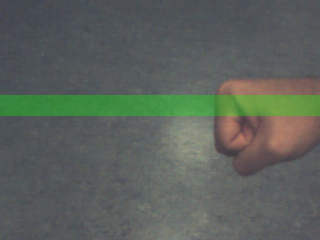
\includegraphics[width=\textwidth]{Chapter4/not-recording}
        \caption{A la espera de entrar en modo grabación.}
        \label{fig:not-recording}
    \end{subfigure}
    ~ %add desired spacing between images, e. g. ~, \quad, \qquad, \hfill etc. 
      %(or a blank line to force the subfigure onto a new line)
    \begin{subfigure}[b]{0.3\textwidth}
        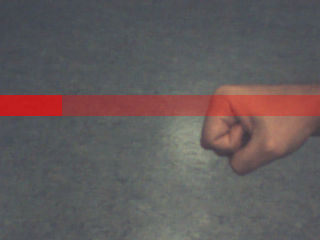
\includegraphics[width=\textwidth]{Chapter4/recording-20}
        \caption{En proceso de grabación, 20\%}
        \label{fig:recording-20}
    \end{subfigure}
    ~ %add desired spacing between images, e. g. ~, \quad, \qquad, \hfill etc. 
    %(or a blank line to force the subfigure onto a new line)
    \begin{subfigure}[b]{0.3\textwidth}
        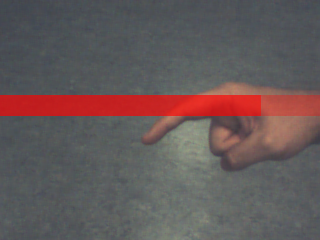
\includegraphics[width=\textwidth]{Chapter4/recording-80}
        \caption{Modo grabación al 80\%}
        \label{fig:recording-80}
    \end{subfigure}
    \caption{Interfaz de usuario para tomar los datos EMG.}\label{fig:obtencion-señal-interfaz}
\end{figure}

\begin{python}[frame=none, numbers=left, label={setup}, caption={Conexión de la \textit{webcam} y la Myo}]
def run(cam_port):
    # Camera set up
    cam = cv2.VideoCapture(cam_port)
    hd.set_up(cam)

    # Myo set up
    m = myo.MyoRaw(sys.argv[1] if len(sys.argv) >= 2
    			    else None)
    m.connect()
    is_disconnected = False

\end{python}



\begin{python}[frame=none, numbers=left,label={data-recorder}, caption={El algoritmo implementado muestra una ventana con la imagen de la \textit{webcam}, cuando el usuario presiona la tecla \textbf{r}(línea 8) se crea un proceso (l. 15) que guarda los
valores que capta la Myo. Se puede diferenciar el ''modo grabación'' cuando la franja cambia de verde \ref{fig:not-recording} a rojo \ref{fig:recording-20} \ref{fig:recording-80} Al pasar un tiempo determinado (l. 19), se procede a recuperar los datos EMG (l.29) así como los de las etiquetas de longitud (l. 30-32). Estos datos son asociados (l.35) y guardados (l.38) }]
def run(cam_port):
...
# Start
while(True):
    # Take a frame form the webcam
    ok, frame = cam.read()
    # Start collecting data when r (recording) is pressed
    if cv2.waitKey(1) & 0xFF == ord('r'):
        # Flag to start the recording's state
        recording = True
        # Set up a thread for recording emg values
        startRecording = time.monotonic()
        # Set up the emg recoerder thread
        emg_queue = Queue()
        p = Process(target=process_run_myo, args=(m, emg_queue, ))
        p.start()
    if recording:
        # Stop recording after hd.RECORD_TIME seconds
        elapsedTime, finished = is_record_finished(startRecording)
        # The guide turns red when recording
        userImg = hd.add_guide(frame.copy(), COLOR_RED)
        # Shows the remaining time until the record ends
        userImgProgress = hd.add_progress(userImg, COLOR_RED,
                                          elapsedTime)
        cv2.imshow('Capture finger lenght', userImgProgress)
        if finished:
            # Save emg values
            p.join()
            emg = emg_queue.get()  # emg is a queue
            fingerList = [queue_length.get()
                             for i in range(0, queue_length.qsize())]
            finger = deque(normalize(fingerList))
            queue_length = Queue()
            # Label each emg value with a finger length [0 - 5]
            dictLabeledData = label_data(emg, finger)
            # Save in a file the data
            num_records += 1
            my_io.save_dict_to(dictLabeledData,
                               name_data_file+str(num_records))
            recording = False
        else:
            p2 = Process(target=process_finger_length,
                         args=(frame, elapsedTime, queue_length, ))
            p2.start()
    # while not recording, show the user-friendly image
    else:
        userImg = hd.add_guide(frame.copy(), (0, 255, 0))
        cv2.imshow('Capture finger lenght', userImg)
cam.release()
cv2.destroyAllWindows()

\end{python}


Por otra parte, el \textit{script hand\_ detection.py} es el encargado de todo lo relativo a las imágenes
captadas por la \textit{webcam}. En el método \ref{finger-length} se aplican distintas técnicas sobre una imagen
RGB para transformarla en una imagen binarizada. Esta imagen es usada en el método \ref{finger-threshold} para
determinar exactamente la longitud del dedo para utilizarla como etiqueta.

\begin{python}[frame=none, numbers=left, label={finger-length},
caption={Este método aplica diversos tratamientos
sobre la imagen para obtener la etiqueta de longitud. Primero se cambia el espectro de color a HSV (línea 3)
\cite{hsv}, se aplica un desenfoque gaussiano (l. 5)\cite{gaussian-blur}. Una vez realizado se aplica a la
imagen un filtro usando un rango de valores (l.7) para obtener la etiqueta de longitud para esa imagen determinada
(l. 11)  }]
def get_finger_strech_and_H_value_from_img(raw_frame):
    # Convert the frame into HSV image
    hsvImg = cv2.cvtColor(raw_frame, cv2.COLOR_BGR2HSV)
    # Apply a blur to clean up the frame
    blurImg = cv2.GaussianBlur(raw_frame, (3, 7), 0)
    # Apply a threshold to try to binarizing the image
    threshImg = cv2.inRange(blurImg, FINGER_MIN, FINGER_MAX)
    # Get the H values for the image
    hValues = mean_h_value_for_img(threshImg)
    # Get the finger lenght
    fingerLen = finger_length(hValues)
    return hValues, fingerLen
\end{python}


\begin{python}[frame=none, numbers=left,label={finger-threshold}, caption={Función que determina en que punto de la empieza el dedo.
Se calcula un límite con el valor de los primeros 40 píxeles que pertenecen al fondo (línea 3), cuando el valor
de la imagen varía significativamente (l. 7) se ha localizado el inicio del dedo (l. 8), y por tanto su longiutd.}]
def finger_length(hValues):
    threshold = sum(hValues[0:40])/40

    for i in range(40, len(hValues)):
        # Find the value that is higher than the threshold
        if hValues[i] < threshold:
            return IMG_WIDTH - i

    # In case of error return -1
    return -1
\end{python}

En las figuras \ref{fig:finger-length-1}, \ref{fig:finger-length-2} y \ref{fig:finger-length-3} se puede ver como, dependiendo de los valores medios de los píxeles comprendidos en la franja que actúa de guía, se determina dónde comienza el dedo. La localización del inicio del dedo se marca en las figuras mediante una línea roja.

\begin{figure}[htp]
  \makebox[\textwidth][c]{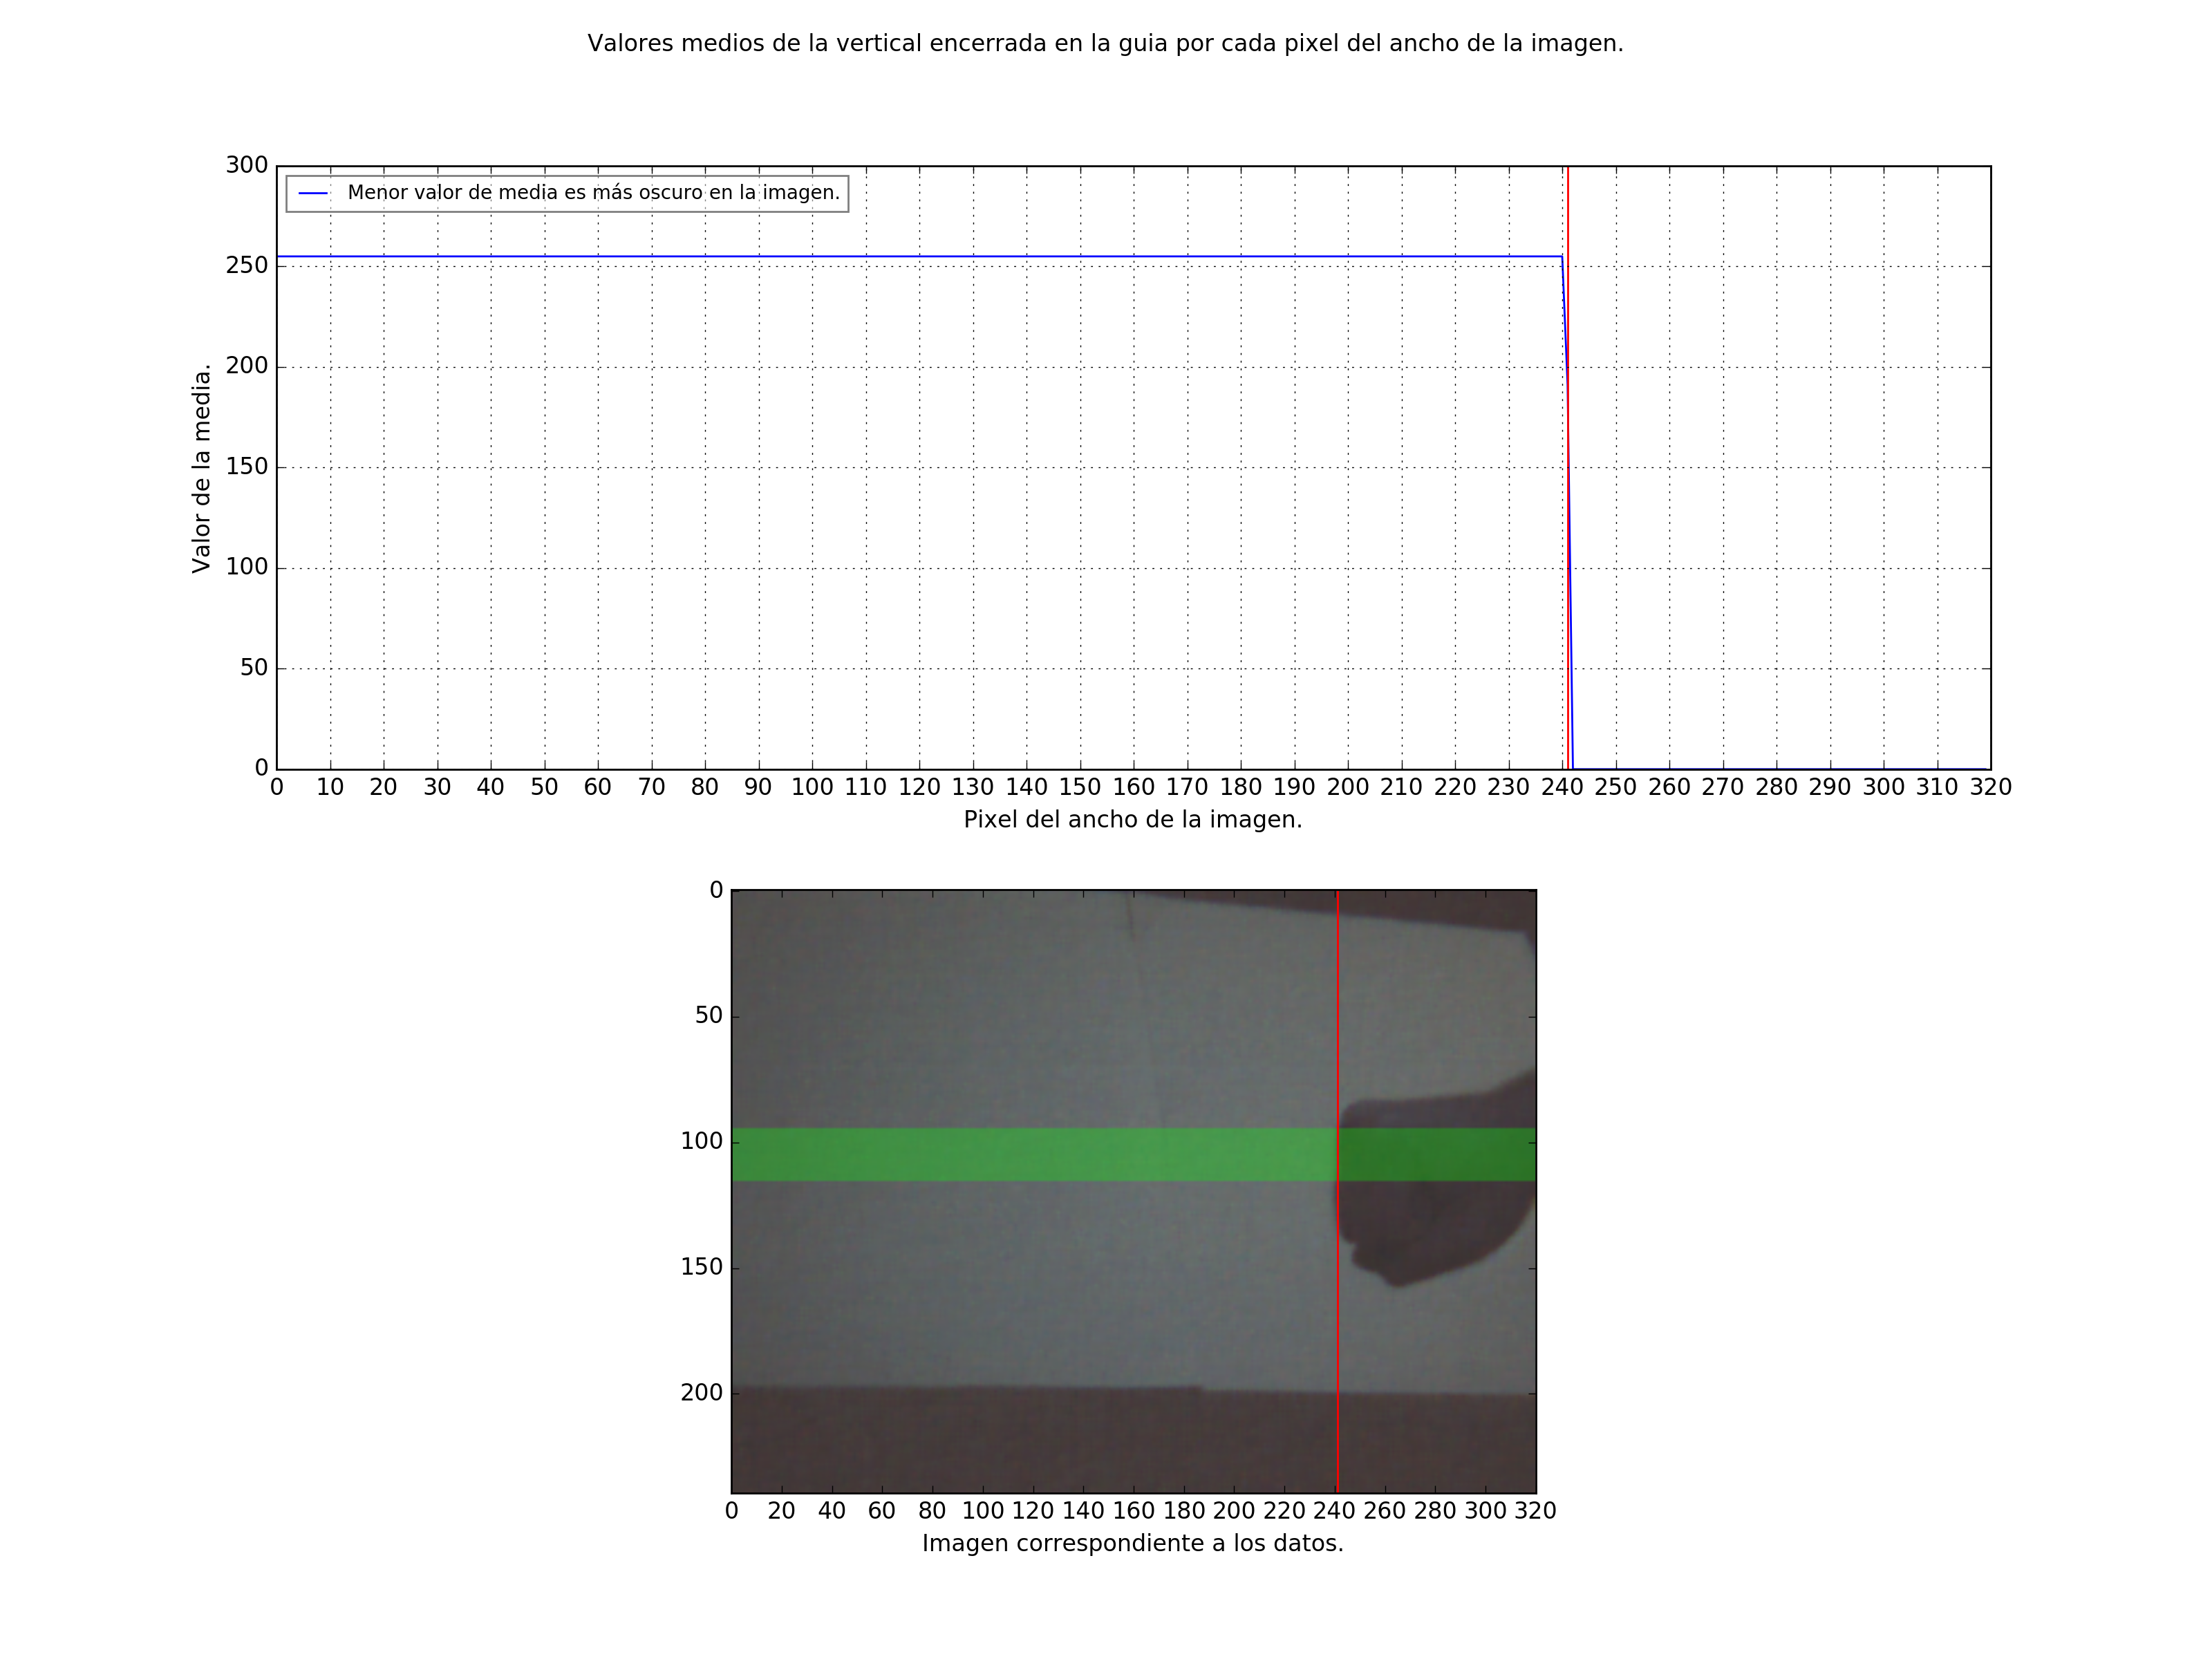
\includegraphics[width=1.8\textwidth]{Chapter4/finger-length-1}}
  \caption{El valor medio es la media de los píxeles comprendidos en la franja dado un píxel de anchura. En la gráfica vemos este valor a lo largo de toda la imagen adjunta.}
\label{fig:finger-length-1}
\end{figure}


\begin{figure}[htp]
  \makebox[\textwidth][c]{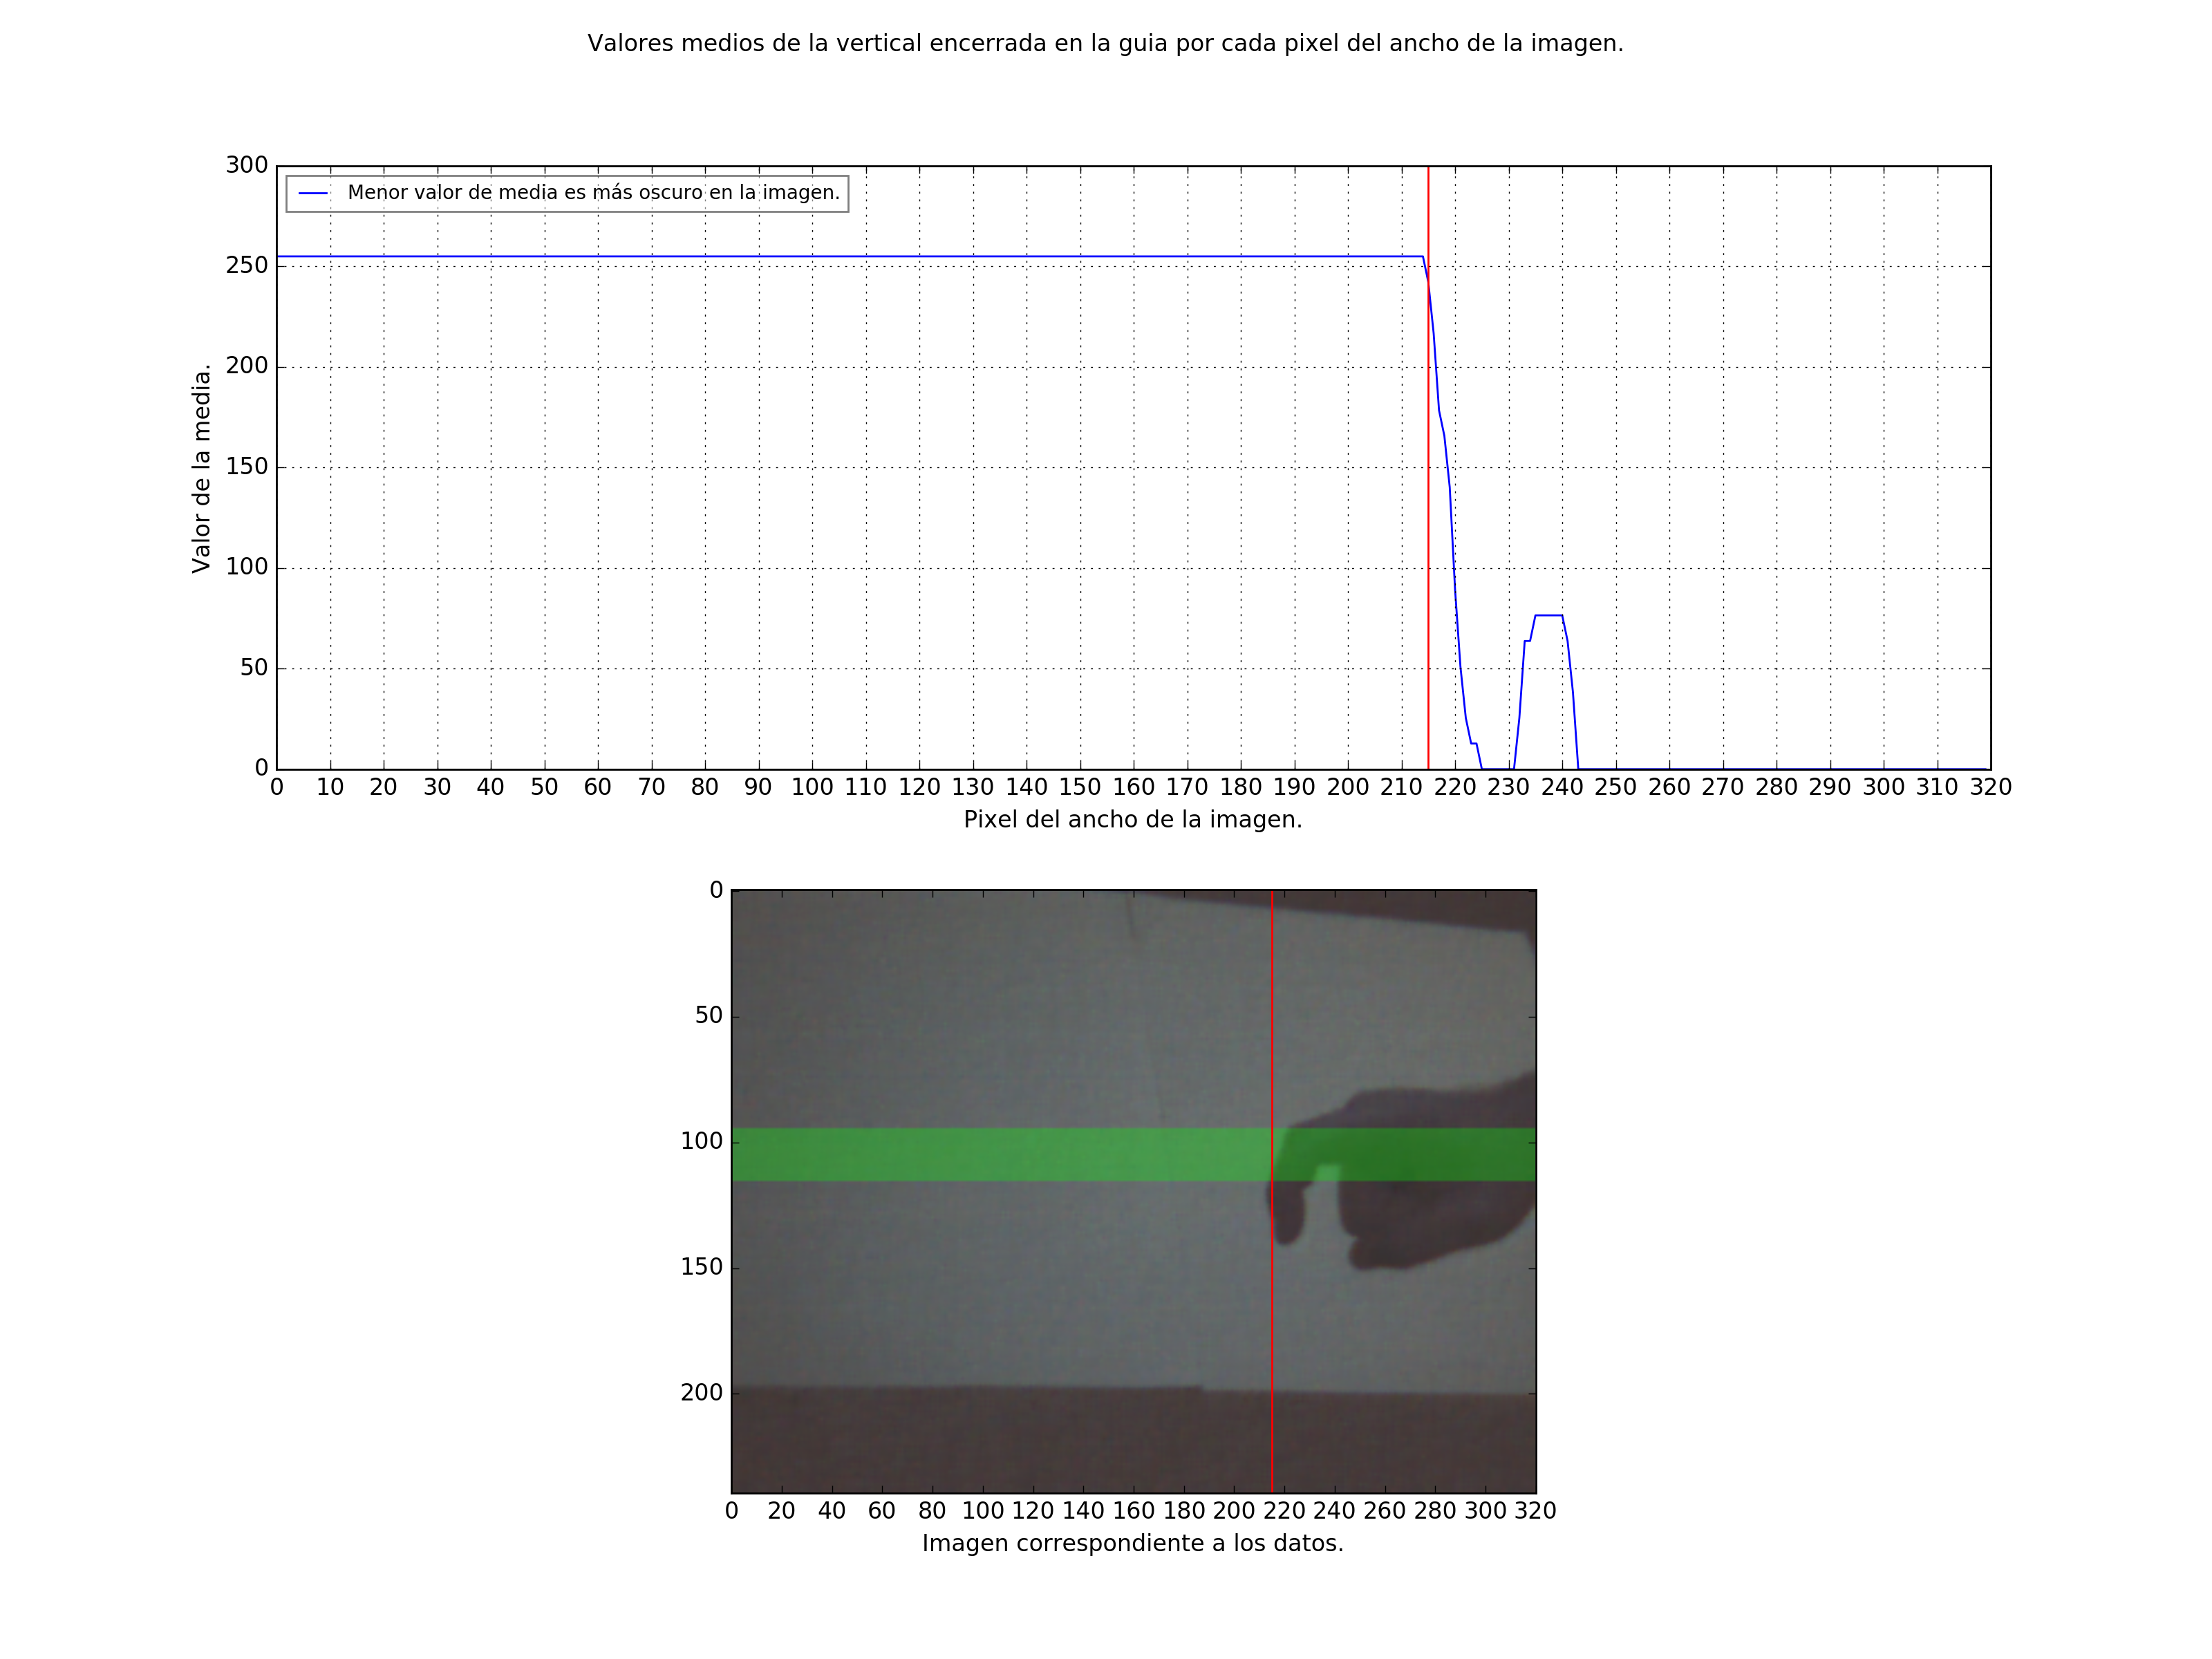
\includegraphics[width=1.8\textwidth]{Chapter4/finger-length-2}}
  \caption{Segunda muestra del código \ref{finger-length} y \ref{finger-threshold}.}
\label{fig:finger-length-2}
\end{figure}



\begin{figure}[htp]
  \makebox[\textwidth][c]{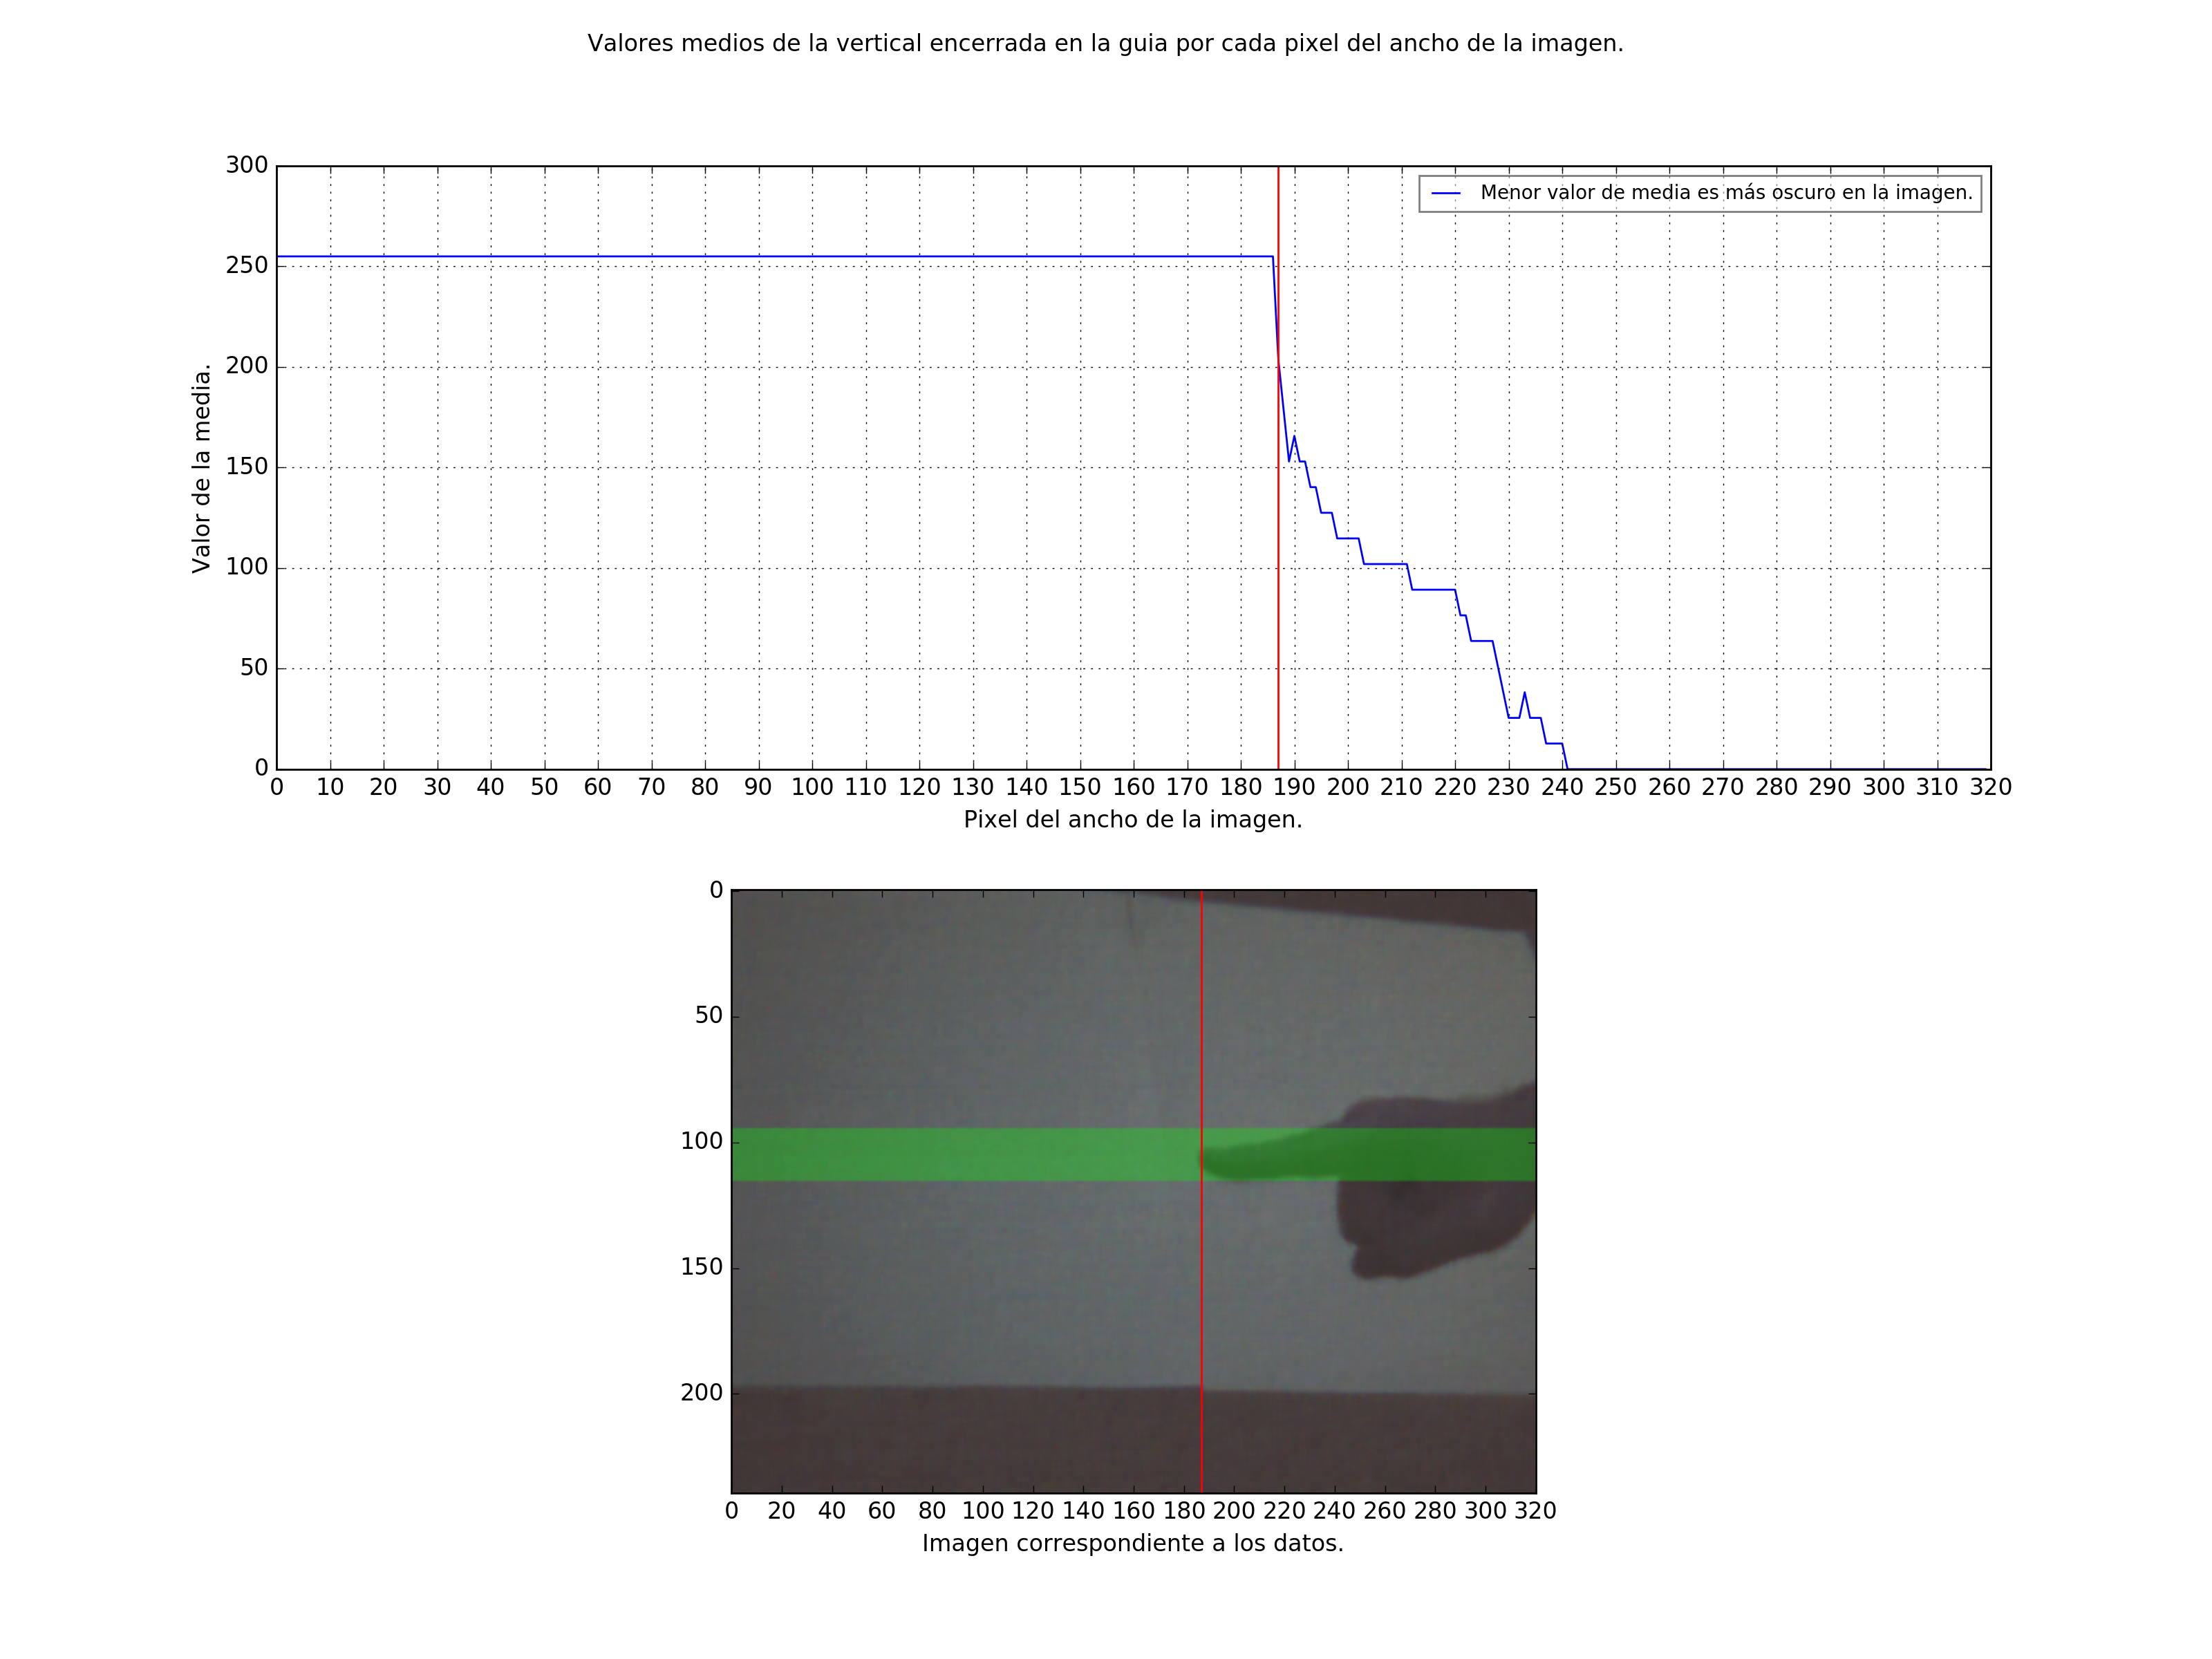
\includegraphics[width=1.8\textwidth]{Chapter4/finger-length-3}}
  \caption{Tercera y última muestra}
\label{fig:finger-length-3}
\end{figure}

\newpage


Mediante el uso de ambos \textit{scripts} obtenemos un fichero separado mediante saltos de línea de la
siguiente forma:

\begin{center}
\textit{label, (int, int, int, int, int, int, int, int)}
\end{center}

Esto es, una etiqueta (\textit{label}) que representa la longitud seguido de 8 números enteros (\textit{int}).
Las etiquetas pueden ser cualquier número entero en el rango de 0 a 5, donde 0 sería el puño cerrado y 5 sería
el dedo en extensión completa. Por otra parte, ocho valores enteros, representan la señal EMG captada por cada
uno de los 8 sensores que posee la Myo. Este fichero con los datos obtenidos de del proceso descrito en %TODO añadir referencia de dónde se explique el proceso de estirar el dedo y coger los datos
serán los datos de entrada para los algoritmos de aprendizaje automático descritos en \ref{sec:clasificación-señales-emg}.








%%%%%%%%%%%%%%%%%%%%%%%%%%%%%%%%%%%%%%%%%%%%%%%%%%%%%%%%%%%%%%%%
%
%
%
%
%        CLASIFICACIÓN DE SEÑALES
%
%
%
%
%%%%%%%%%%%%%%%%%%%%%%%%%%%%%%%%%%%%%%%%%%%%%%%%%%%%%%%%%%%%%%%%


\section{Clasificación de señales EMG}
\label{sec:clasificación-señales-emg}


Para lograr que la prótesis responda correctamente a los movimientos del usuario mediante la Myo, se ha diseñado
un modelo %TODO cambiar a plural si decido añadir más algoritmos
basado en \textit{Deep learning} %TODO añadir referencia deeplearning
utilizando las herramientas \textit{software}: \textit{nolearn} \ref{subs:nolearn}, \textit{lasagne} \ref{subs:lasagne} y \textit{scikit-learn} \ref{subs:scikit-learn}.
%TODO añadir más frameworks si añado más cosas



Para acceder al conjunto de datos de entrenamiento se ha desarrollado un programa auxiliar para ello.
Desde \textit{dataset.py} es posible recuperar los datos mediante el uso del método que podemos ver en
ref{load-dataset}.

Este método es de gran importancia puesto que la correcta carga de los datos es fundamental para el buen
funcionamiento del la red neuronal. En las líneas 6-15 se lee el fichero creado por \textit{data\_recorder.py}
\ref{data-recorder}. Como existe la posibilidad de que los datos estén ordenados de alguna forma, se debe aplicar
una permutación(líneas 18-22). Por último, se reserva una cantidad de datos fija (2000 en este caso) como conjunto
de validación (líneas 25-26). Este conjunto permite determinar la tasa de aciertos real del modelo entrenado, pues nunca formara parte del propio entrenamiento.

\begin{python}[frame=none, numbers=left,label={load-dataset}, caption={Método encargado de preparar los conjuntos de validación y entrenamiento para la red neuronal.}]
 def load_dataset():
    list_data = my_io.readFile('./Data/all_data')
    X = []
    y = []

    for data in list_data:
        y.append(eval(data[:1]))
        aux = data[4:-1].split(',')
        for i in range(len(aux)):
            aux2 = np.empty(8, dtype=np.int64)
            aux2[i] = aux[i]
        X.append(aux2)

    X = np.array(X, dtype=np.float32)
    y = np.array(y, dtype=np.int32)

    # Declare a random number generator
    rng = np.random.RandomState(seed=0)

    # Shuffle the data the right way to avoid missleading label-emg
    permutation = rng.permutation(len(X))
    X, y = X[permutation], y[permutation]

    # We reserve the last 2000 training examples for validation.
    X_train, X_val = X[:-2000], X[-2000:]
    y_train, y_val = y[:-2000], y[-2000:]

    # return all the arrays in order, as expected in main().
    return X_train, y_train, X_val, y_val

 \end{python}

Los conjuntos de datos serán utilizados por el fichero \textit{neural\_network.py} \ref{neural-network}. Este
fichero contien todo lo referente al proceso de aprendizaje, desde la construcción de la arquitectura de la red neuronal(línea 7) hasta el proceso de aprendizaje (l. 11) y la evaluación del modelo (l. 19)

\begin{python}[frame=none, numbers=left, label={neural-network},
caption={Declaración, aprendizaje y evaluación de la red neuronal}]
def main(num_epochs=500):
    # Load the dataset
    print("Loading data...")
    X, y, X_val, y_val = dataset.load_dataset_and_validationset()

    # Building the network
    nn = build_nn()

    # Begin the training phase
    tic = my_time_utils.begin()
    nn.fit(X, y)

    # Show how much time does it take the training phase
    print('Finished fitting in '
          + str(my_time_utils.elapsed_time(tic)) + 'seconds\n')

    # Show the accuracy of the model
    print('Scoring...')
    print(round(nn.score(X_val, y_val)*100, 4), '%',)

\end{python}

La arquitectura de la red neuronal \ref{nn-arquitecture} se compone de una capa de entrada, una capa de salida y de 3 capas ocultas

\begin{python}[frame=none, numbers=left, label={nn-arquitecture}, caption={Arquitectura y parámetros de la red neuronal}]
def build_nn():
    num_features = 8
    num_classes = 6

    layers = [  # 5 layers: 3 hidden layers
              ('input', InputLayer),
              ('dense0', DenseLayer),
              ('dropout0', DropoutLayer),
              ('dense1', DenseLayer),
              ('dropout1', DropoutLayer),
              ('dense2', DenseLayer),
              ('dropout2', DropoutLayer),
              ('output', DenseLayer)]
    # layer parameters:
    net = NeuralNet(layers=layers,
                    # Input
                    input_shape=(None, num_features),
                    # Dense0
                    dense0_nonlinearity=tanh,
                    dense0_num_units=200,
                    dropout0_p=0.4,
                    # Dense1
                    dense1_nonlinearity=tanh,
                    dense1_num_units=200,
                    dropout1_p=0.2,
                    # Dense2
                    dense2_num_units=200,
                    dense2_nonlinearity=tanh,
                    dropout2_p=0.2,
                    # Output
                    output_num_units=num_classes,
                    output_nonlinearity=softmax,

                    update=nesterov_momentum,
                    update_learning_rate=0.01,
                    update_momentum=0.9,

                    verbose=1,
                    on_training_finished=[report.PlotLossesAccuracy(
                                          figsize=(16, 12), dpi=200)],
                    max_epochs=500)

    return net
\end{python}

Además de la arquitectura de la red en \ref{nn-arquitecture}, podemos ver a partir de la línea 17, una
serie de parámetros. Estos parámetros configuran el comportamiento y definen cómo aprende la red neuronal:

\begin{itemize}

\item \textit{Input\_shape}: define los datos de entrada de la red. En este caso, los datos serían los 8 valores
captados por la Myo.

%TODO añadir referencia a la explicación de no linearidad
\item \textit{DenseX\_nonlinearity}: atribuye una función de activación no linear a la capa oculta \textit{X}.

\item \textit{DenseX\_num\_units}: número de unidades (neurones) que posee la capa oculta \textit{X}.

\item \textit{Update}: estas funciones afectan al cálculo del \textit{training rate} durante todo el proceso
de entrenamiento/aprendizaje.

\item \textit{{Update\_training\_rate}}: modifica el tamaño de los pasos del aprendizaje.

\item \textit{Update\_momentum}: permite suavizar los valores oscilantes de los errores.

\item \textit{Verboese}: muestra por pantalla valores como el error y los aciertos por cada iteración.

\item \textit{On\_training\_finished}: permite activar funciones o procedimientos al terminar el entrenamiento.

\item \textit{Max\_epoch}: número de iteraciones máximas que puede llevar el entrenamiento de la red.

\end{itemize}

%TODO concluir el apartado del código de la red neuronal



%%%%%%%%%%%%%%%%%%%%%%%%%%%%%%%%%%%%%%%%%%%%%%%%%%%%%%%%%%%%%%%%
%
%
%        EXPERIMENTACIÓN
%
%
%%%%%%%%%%%%%%%%%%%%%%%%%%%%%%%%%%%%%%%%%%%%%%%%%%%%%%%%%%%%%%%%

\newpage

\section{Experimentación}
\label{sec:experimentación}


Las redes neuronales pueden llegar a alcanzar millones de hiper-parámetros \cite{NovikovPOV15} y es necesario
probar diversas calibraciones. En esta sección se expondrán las pruebas realizadas con la red neuronal definida
en \ref{nn-arquitecture}.

El primer parámetro a probar será \textit{update} sin modificar ningún otro de los parámetro descritos en \ref{nn-arquitecture}. Los resultados que se muestran en \ref{tab:update} son los resultados del aprendizaje sobre el
conjunto de datos de validación


\begin{table}[htp]
\caption{Porcentaje de aciertos obtenido usando el conjunto de entrenamiento según el algoritmo utilizado como
\textit{update}. El mejor resultado está marcado en negrita.}
\label{tab:update}
\centering
\begin{tabular}{l c c c c}
\toprule
& \textbf{rmsprop} & \textbf{adagrad} & \textbf{nesterov-momentum}  &   \textbf{adam}  \\
\midrule
Tasa de aciertos (\%) & 47.25 & 52.89 & \textbf{58.25} & 48.96   \\
\bottomrule\\

\end{tabular}
\end{table}


\begin{table}[htp]
\label{tab:aciertos}
\centering
\begin{tabular}{l c c c c }
\toprule
 & \textbf{momentum} &  \textbf{sgd}  &  \textbf{adamax}  & \textbf{adadelta}\\
\midrule
Tasa de aciertos (\%) & 56.50 & 48.84 & 56.90 & 47.08 \\
\bottomrule\\

\end{tabular}
\end{table}



En las siguientes pruebas se utilizará \textit{nesterov-momentum} como función de actualización por haber conseguido la mayor tasa de aciertos (58.25\%). 

Cada una de las capas ocultas de la red puede implementar una función de activación no lineal\cite{nonlinearities}. La tabla \ref{tab:nonlinearities} es el resultado de aplicar \textit{grid search} sobre las funciones \textit{verify, tanh y sigmoid} en cada capa oculta de la red neuronal. De ella, se puede extraer que la combinación \textit{rectify-rectify-rectify} es la que presenta mejores resultados (40.36\%)

\begin{table}[htp]
\caption{Porcentaje de aciertos sobre el conjunto de entrenamiento mediante la permutación de las funciones \textit{verify}, \textit{tanh} y \textit{sigmoid}. En negrita se marca el mejor resultado.}
\label{tab:nonlinearities}
\centering
\begin{tabular}{c c c c c}

\toprule
\textbf{Capa oculta 1} & \textbf{Capa oculta 2} & \textbf{Capa oculta 3} & \textbf{Precisión (\%)} & \textbf{std} \\
\midrule
tanh & tanh & tanh & 52.16 & 0.00563   \\
tanh & sigmoid & tanh & 51.51 & 0.00660   \\
tanh & rectify & tanh & 54.53 & 0.00794   \\
tanh & tanh & sigmoid & 47.81 & 0.00565   \\
tanh & sigmoid & sigmoid & 46.35 & 0.01223   \\
tanh & rectify & sigmoid & 50.89 & 0.00871   \\
tanh & tanh & rectify & 52.91 & 0.00671   \\
tanh & sigmoid & rectify & 52.64 & 0.00696   \\
tanh & rectify & rectify & 55.91 & 0.00858   \\
sigmoid & tanh & tanh & 46.30 & 0.01287   \\
sigmoid & sigmoid & tanh & 46.02 & 0.01117   \\
sigmoid & rectify & tanh & 49.95 & 0.00885   \\
sigmoid & tanh & sigmoid & 43.9 & 0.00864   \\
sigmoid & sigmoid & sigmoid & 41.81 & 0.00656   \\
sigmoid & rectify & sigmoid & 46.51 & 0.01078   \\
sigmoid & tanh & rectify & 47.44 & 0.00752   \\
sigmoid & sigmoid & rectify & 46.31 & 0.01228   \\
sigmoid & rectify & rectify & 51.21 & 0.00854   \\
rectify & tanh & tanh & 49.98 & 0.00526   \\
rectify & sigmoid & tanh & 50.31 & 0.00916   \\
rectify & rectify & tanh & 54.37 & 0.00501   \\
rectify & tanh & sigmoid & 49.09 & 0.01037   \\
rectify & sigmoid & sigmoid & 46.23 & 0.00888   \\
rectify & rectify & sigmoid & 51.22 & 0.00635   \\
rectify & tanh & rectify & 55.07 & 0.01142   \\
rectify & sigmoid & rectify & 51.54 & 0.00993   \\
\textbf{rectify} & \textbf{rectify} & \textbf{rectify} & \textbf{56.77} & \textbf{0.00961}   \\


\bottomrule\\
\end{tabular}
\end{table}





\newpage






El siguiente experimento se realizará sobre el parámetro que controla el número de unidades (neuronas) de cada una de las capas ocultas de la red neuronal y el parámetro \textit{dropout} \ref{subs:dropout}:

\begin{itemize}

	\item Perfil bajo: 200 neuronas por capa y 0.2 de \textit{dropout}.

	\item Perfil intermedio: 1200 neuronas por capa y 0.4-0.5 de \textit{dropout}.

	\item Perfil alto: 10000 neuronas por capa y 0.8-0.9 de \textit{dropoout}.

\end{itemize}


\begin{table}[htp]
\caption{Experimentación con el número de unidades (neuronas) y \textit{dropout}. Marcado en negrita está el mejor resultado.}
\centering
\begin{tabular}{l c c c}
\toprule
& \textbf{Neuronas} & \textbf{Dropout} & \textbf{Precisión de validación (\%)} \\
\midrule
\textbf{Perfil bajo}  & 200   &  0.2  & 55.25  \\
\textbf{Perfil medio} & \textbf{1200}  &  \textbf{0.4}  & \textbf{61.10}  \\
\textbf{Perfil alto}  & 4500  &  0.8  & 45.05  \\

\bottomrule\\

\end{tabular}
\label{tab:perfil}
\end{table}


En la tabla \ref{tab:perfil} el perfil alto usa 4500 neuronas cuando debería ser una prueba con 10000
o más neuronas, esto es debido a limitaciones de la tarjeta gráfica del equipo utilizado para las pruebas (NVIDIA GT 540M).


En la columna de precisión de validación, podemos ver la tasa de aciertos que logra el modelo con datos con los que
no ha sido entrenado. Vemos que un mayor número de neuronas no implica una mayor tasa de aciertos, pero se puede observar que 1200 neuronas con 0.4 de \textit{dropout} funcionan mejor que 200 neuronas con 0.2 de \textit{dropout}.
La configuración del perfil medio es la que se usará en la siguiente y última prueba.


El último parámetro a probar es el \textit{learning rate}, la tabla \ref{tab:learning-rate}

\begin{table}[htp]
\caption{Experimentación con el parámetro \textit{learning rate}. En negrita se marca el mejor resultado.}
\centering
\begin{tabular}{c c}
\toprule
\textbf{Learning rate} &  \textbf{Precisión de validación (\%)} \\
\midrule
  0.1    &  44.00  \\
  \textbf{0.01}   &  \textbf{61.10}  \\
  0.001  &  43.25  \\

\bottomrule\\

\end{tabular}
\label{tab:learning-rate}
\end{table}







\newpage




\subsection{Modelo final}

Tras el proceso de experimentación, los parámetros que se usarán en el apartado de resultados (\ref{subs:resultados}) son los que se muestran a continuación en \ref{parametros-finales}.

\begin{python}[frame=none, numbers=left, label={parametros-finales}, caption={Configuración de las capas de la red neuronal y sus parámetros finales marcados en negrita}]
num_features = 8
num_classes = 6

layers = [  # 5 layers: 3 hidden layers
          ('input', InputLayer),
          ('dense0', DenseLayer),
          ('dropout0', DropoutLayer),
          ('dense1', DenseLayer),
          ('dropout1', DropoutLayer),
          ('dense2', DenseLayer),
          ('dropout2', DropoutLayer),
          ('output', DenseLayer)]
# layer parameters:
net = NeuralNet(layers=layers,
                # Input
                input_shape=(None, num_features),
                # Dense0
                dense0_nonlinearity=rectify,
                dense0_num_units=1200,
                dropout0_p=0.4,
                # Dense1
                dense1_nonlinearity=rectify,
                dense1_num_units=1200,
                dropout1_p=0.4,
                # Dense2
                dense2_num_units=1200,
                dense2_nonlinearity=rectify,
                dropout2_p=0.4,
                # Output
                output_num_units=num_classes,
                output_nonlinearity=softmax,

                update=nesterov_momentum,
                update_learning_rate=0.01,

                max_epochs=500)
\end{python}

\subsection{Resultados}
\label{subs:resultados}

El rendimiento del modelo, como se ha explicado anteriormente, se determinará mediante el conjunto de validación
compuesto por 2000 de los 26540 conjunto total de datos disponibles. Remarcar de nuevo, que este grupo de datos no
ha sido utilizado en ningún momento en el proceso de aprendizaje, por lo cual, todos los datos son nuevos para el
modelo.

El primer resultado se muestra en la figura \ref{fig:confusion-matrix}. Esta matriz permite ver de forma gráfica el
resultado de las predicciones. A la matriz le acompaña una barra de colores, donde el color más cálido (marrón en
este caso) indica una mayor tasa de coincidencia de índices columna-fila. En contraposición, el color frío indica
un menor ratio. Idealmente, la matriz debería mostrar en su diagonal secundaria los tonos cálidos, indicando que las predicciones son correctas.


\begin{figure}[htp]
  \centering
    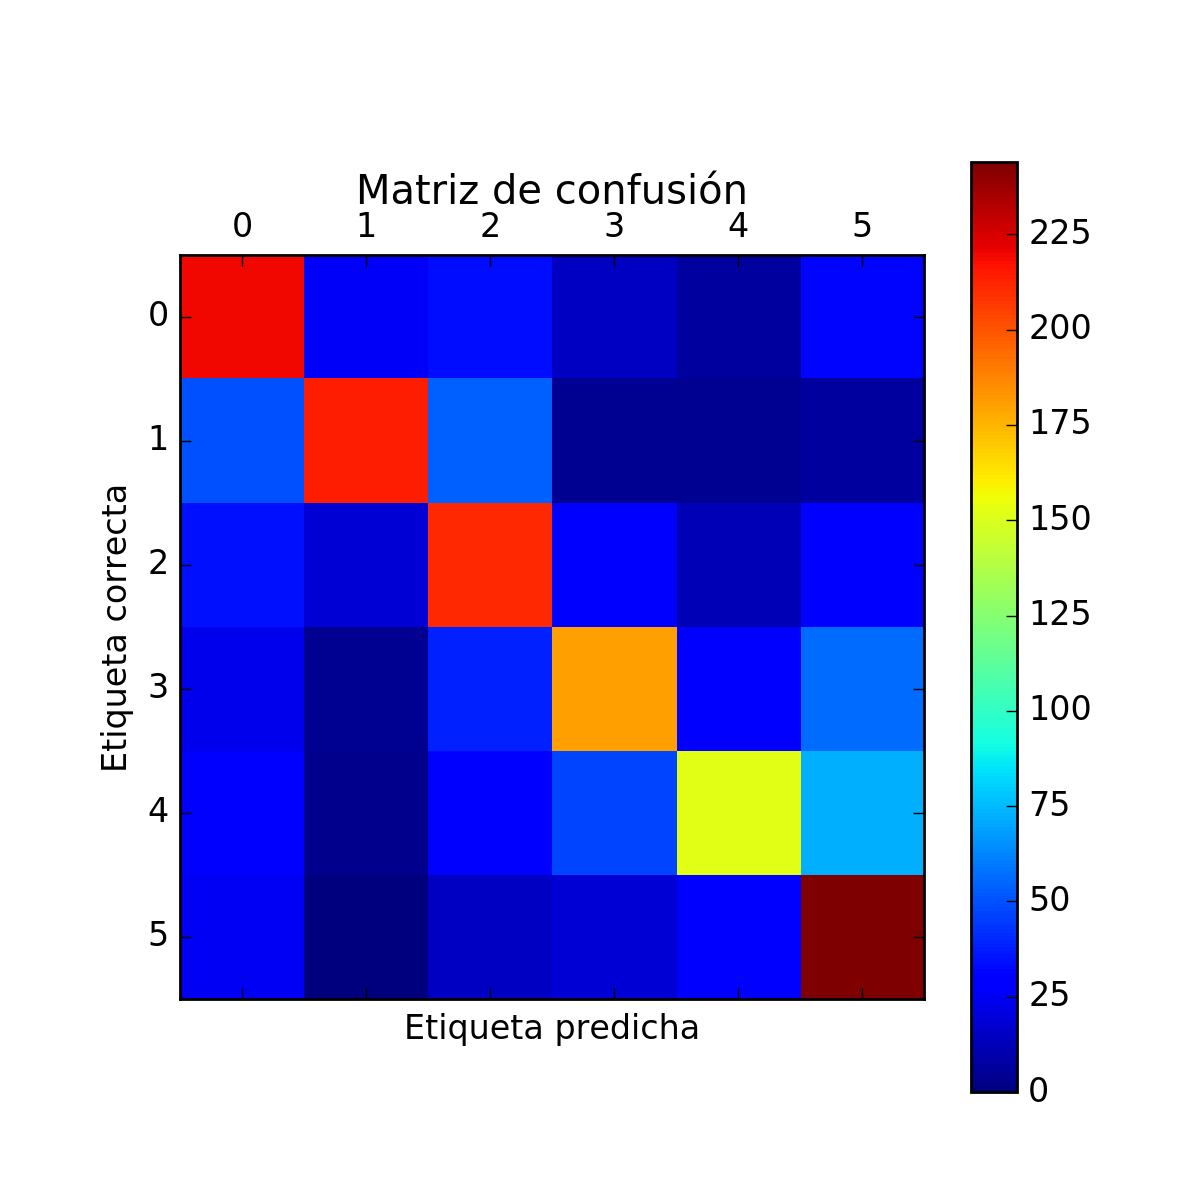
\includegraphics[width=0.8\textwidth]{Chapter4/ultimo-test-matriz}
  \caption{Matriz de confusión del modelo de red neuronal final.}
\label{fig:confusion-matrix}
\end{figure}

La precisión de un modelo no debe ser nunca el único indicador de calidad o rendimiento de un modelo de aprendizaje,
puesto que en ámbitos como el de, por ejemplo, la medicina obtener un falso positivo o un falso negativo, puede ser un grave error. Por ello, se ha incluido un informe con datos sobre además de la precisión, las medidas de exhaustividad (\textit{recall}, en inglés) que mide el verdadero ratio de positivos (es el verdaderos positivos dividido por los verdaderos positivos y falsos negativos)  y valor-F (\textit{F1 score}, en inglés) que es una media entre la exhaustividad y la precisión, concretamente se mide como:

\begin{equation}
2*\frac{Precisi\acute{o}n*Exhaustividad}{Precisi\acute{o}n+Exhaustividad}
\end{equation}



\begin{table}[htp]
\caption{Tabla con un resumen de distintos criterios de evaluación sobre los aciertos de cada etiqueta.}
\label{tab:report}
\centering
\begin{tabular}{l c c c}

\toprule
	&	\textbf{Precisión}	&	\textbf{Exhaustividad}		& \textbf{Valor-F} \\
\midrule
Etiqueta 0		&	0.57	&	0.66	&	0.61			\\
Etiqueta 1		&	0.80	&	0.64	&	0.71		\\
Etiqueta 2		&	0.55	&	0.63	&	0.59		\\
Etiqueta 3		&	0.61	&	0.54	&	0.58		\\
Etiqueta 4		&	0.65	&	0.46	&	0.54		\\
Etiqueta 5		&	0.55	&	0.73	&	0.63		\\
\midrule
\textbf{Media}		&	0.62	&	0.61	&	0.61		\\
\bottomrule\\
\end{tabular}
\end{table}
